\chapter{Appendix: Anforderungen}
\label{ch:appendix:requirements}
% Die folgenden Definitionen wurden wörtlich aus der ISO-Norm 25010 (\cite{ISO25010}) entnommen:
%
% \section*{functional suitability}
% "degree to which a product or system provides functions that meet stated and implied needs when used under specified conditions"
% \begin{description}
%   \item[functional completeness] "degree to which the set of functions covers all the specified tasks and user objectives"
%   \item[functional correctness] "degree to which a product or system provides the correct results with the needed degree of precision"
%   \item[functional appropriateness] "degree to which the functions facilitate the accomplishment of specified tasks and objectives"
% \end{description}
%
% \section*{performance efficiency}
% "performance relative to the amount of resources used under stated conditions"
% \begin{description}
%   \item[time behaviour] "degree to which the response and processing times and throughput rates of a product or system, when performing its functions, meet requirements"
%   \item[resource utilization] "degree to which the amounts and types of resources used by a product or system, when performing its functions, meet requirements"
%   \item[capacity] "degree to which the maximum limits of a product or system parameter meet requirements"
% \end{description}
%
% \section*{compatibility}
% "degree to which a product, system or component can exchange information with other products, systems or components, and/or perform its required functions, while sharing the same hardware or software environment"
% \begin{description}
%   \item[co-existence] "degree to which a product can perform its required functions efficiently while sharing a common environment and resources with other products, without detrimental impact on any other product"
%   \item[interoperability] "degree to which two or more systems, products or components can exchange information and use the information that has been exchanged"
% \end{description}
%
% \section*{usability}
% "degree to which a product or system can be used by specified users to achieve specified goals with effectiveness, efficiency and satisfaction in a specified context of use"
% \begin{description}
%   \item[appropriateness recognizability] "degree to which users can recognize whether a product or system is appropriate for their needs"
%   \item[learnability] "degree to which a product or system can be used by specified users to achieve specified goals of learning to use the product or system with effectiveness, efficiency, freedom from risk and satisfaction in a specified context of use"
%   \item[operability] "degree to which a product or system has attributes that make it easy to operate and control"
%   \item[user interface aesthetics] "degree to which a user interface enables pleasing and satisfying interaction for the user"
%   \item[accessibility] "degree to which a product or system can be used by people with the widest range of characteristics and capabilities to achieve a specified goal in a specified context of use"
% \end{description}
%
% \section*{reliability}
% "degree to which a system, product or component performs specified functions under specified conditions for a specified period of time"
% \begin{description}
%   \item[maturity] "degree to which a system, product or component meets needs for reliability under normal operation"
%   \item[availability] "degree to which a system, product or component is operational and accessible when required for use"
%   \item[fault tolerance] "degree to which a system, product or component operates as intended despite the presence of hardware or software faults"
%   \item[recoverability] "degree to which, in the event of an interruption or a failure, a product or system can recover the data directly affected and re-establish the desired state of the system"
%   \item[]
% \end{description}
%
% \section*{security}
% "degree to which a product or system protects information and data so that persons or other products or systems have the degree of data access appropriate to their types and levels of authorization"
% \begin{description}
%   \item[confidentiality] "degree to which a product or system ensures that data are accessible only to those authorized to have access"
%   \item[integrity] "degree to which a system, product or component prevents unauthorized access to, or modification of, computer programs or data"
%   \item[non-repudiation] "degree to which actions or events can be proven to have taken place, so that the events or actions cannot be repudiated later"
%   \item[accountability] "degree to which the actions of an entity can be traced uniquely to the entity"
%   \item[authenticity] "degree to which the identity of a subject or resource can be proved to be the one claimed"
% \end{description}
%
% \section*{maintainability}
% "degree of effectiveness and efficiency with which a product or system can be modified by the intended maintainers"
% \begin{description}
%   \item[modularity] "degree to which a system or computer program is composed of discrete components such that a change to one component has minimal impact on other components"
%   \item[reusability] "degree to which an asset can be used in more than one system, or in building other assets"
%   \item[analysability] "degree of effectiveness and efficiency with which it is possible to assess the impact on a product or system of an intended change to one or more of its parts, or to diagnose a product for deficiencies or causes of failures, or to identify parts to be modified"
%   \item[modifiability] "degree to which a product or system can be effectively and efficiently modified without introducing defects or degrading existing product quality"
%   \item[testability] "degree of effectiveness and efficiency with which test criteria can be established for a system, product or component and tests can be performed to determine whether those criteria have been met"
% \end{description}
%
% \section*{portability}
% "degree of effectiveness and efficiency with which a system, product or component can be transferred from one hardware, software or other operational or usage environment to another"
% \begin{description}
%   \item[adaptability] "degree to which a product or system can effectively and efficiently be adapted for different or evolving hardware, software or other operational or usage environments"
%   \item[installability] "degree of effectiveness and efficiency with which a product or system can be successfully installed and/or uninstalled in a specified environment"
%   \item[replaceability] degree to which a product can replace another specified software product for the same purpose in the same environment
% \end{description}


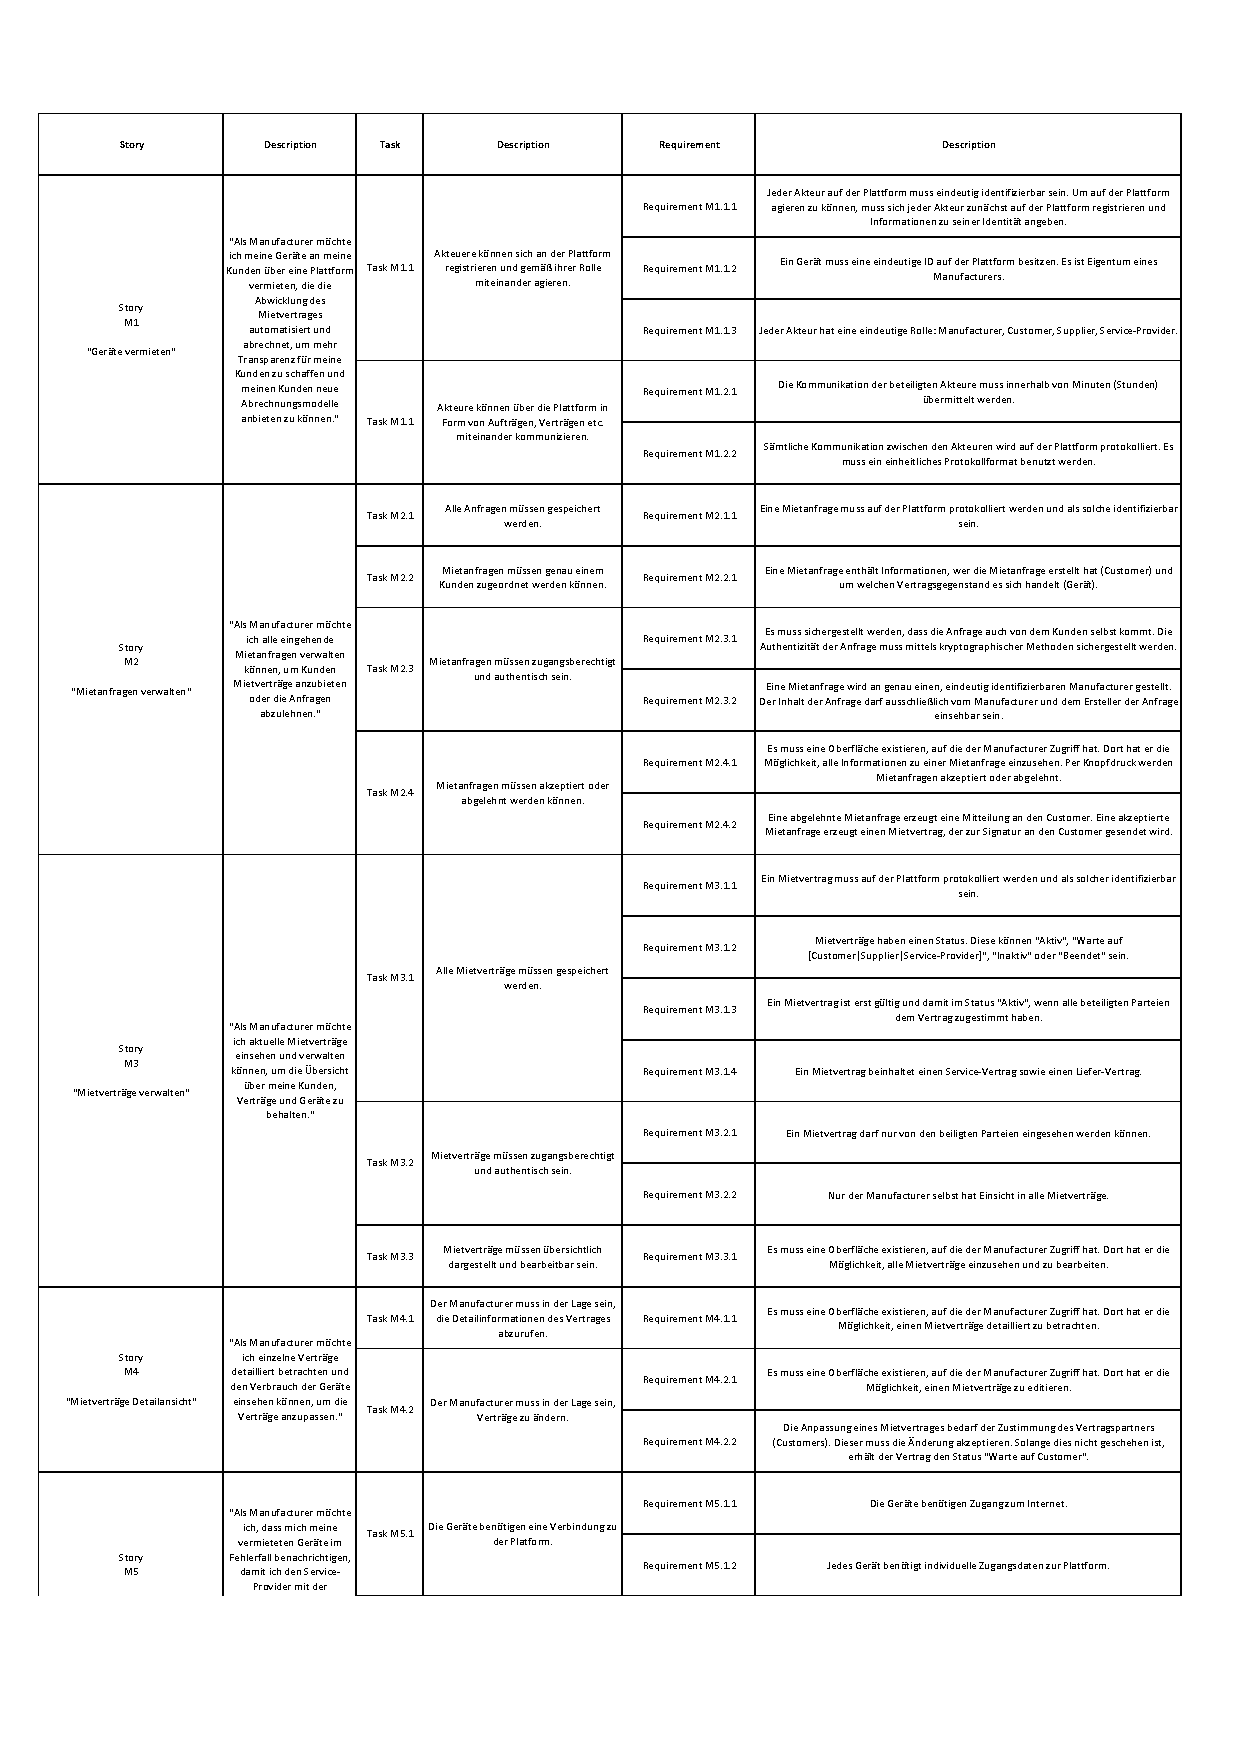
\includepdf[pages=-]{gfx/Requirements_v1.pdf}


\chapter{Appendix: Code}
\label{ch:appendix:code}

\lstinputlisting{gfx/code/RentalProvider.sol}
\lstinputlisting{gfx/code/PaymentProvider.sol}
\lstinputlisting{gfx/code/IdentityProvider.sol}
